 \documentclass{jacow}
\usepackage{graphicx}
\usepackage{booktabs}
\usepackage{bigints}
\usepackage{url}
\usepackage{grffile} % can use other graphics extensions (e.g. doesn't error for example.0.1.png)
\usepackage{float} % \begin{figure}[H] makes figures not float (really really here)
\usepackage{array}
\newcolumntype{P}[1]{>{\centering\arraybackslash\vspace{-2mm}}p{#1}}


\usepackage{svg}
%%
%%   VARIABLE HEIGHT FOR THE TITLE BOX (default 35mm)
%%

\setlength{\titleblockheight}{27mm}

\begin{document}
\title{THE ADVANCEMENT OF COOLING ABSORBERS IN COSY INFINITY\thanks{Work supported by the U.S. Department of Energy}}

\author{J. Kunz, P. Snopok\thanks{psnopok@iit.edu}, Illinois Institute of Technology, Chicago, IL 60616, USA \\
M. Berz, K. Makino, Michigan State University, East Lansing, MI 48824, USA}

\maketitle

\begin{abstract}
COSY Infinity is an arbitrary-order beam dynamics simulation and analysis code. It can determine high-order transfer maps of combinations of particle optical elements of arbitrary field configurations. For precision modeling, design, and optimization of next-generation muon beam facilities, its features make it a very attractive code. New features are being developed for inclusion in COSY to follow the distribution of charged particles through matter. To study in detail some of the properties of muons passing through material, the transfer map approach alone is not sufficient. The interplay of beam optics and atomic processes must be studied by a hybrid transfer map--Monte-Carlo approach in which transfer map methods describe the average behavior of the particles in the accelerator channel including energy loss, and Monte-Carlo methods are used to provide small corrections to the predictions of the transfer map accounting for the stochastic nature of scattering and straggling of particles. The advantage of the new approach is that it is very efficient in that the vast majority of the dynamics is represented by fast application of the high-order transfer map of an entire element and accumulated stochastic effects as well as possible particle decay. The gains in speed are expected to simplify the optimization of muon cooling channels which are usually very computationally demanding due to the need to repeatedly run large numbers of particles through large numbers of configurations. Progress on the development of the required algorithms is reported.
\end{abstract}

\section{INTRODUCTION}

Muons are tertiary production particles (protons $\rightarrow$ pions $\rightarrow$ muons) and high-intensity collection requires a large initial phase space volume. The resultant spray of muons must be amassed, focused, and accelerated well within the muon lifetime (2.2~$\mu$s in the rest frame). The only technique fast enough to reduce the beam size within the muon lifetime is ionization cooling. When muons traverse a material, energy is lost in both the longitudinal and transverse directions due to ionization. The energy is then restored in the longitudinal direction only, leading to an overall reduction in the transverse beam size (cooling). In order to achieve cooling in the longitudinal direction, emittance exchange is used, usually involving wedge-shaped absorbers. For some applications such as a high-energy high-luminosity muon collider, cooling needs to be very aggressive: six-dimensional emittance reduction over six orders of magnitude is required to reach design goals.

In order to carefully simulate the effect of the absorbers on the beam, one needs to take into account both deterministic and stochastic effects in the ionization energy loss. The deterministic effects in the form of the Bethe-Bloch formula with various theoretical and experimental corrections fit well into the transfer map methods approach, where the effect of the lattice on the particles is evaluated first by producing the so-called transfer map, and then is applied to a given initial distribution of particles. The arbitrary-order simulation code COSY Infinity \cite{COSY} is a key representative of transfer map codes. COSY was chosen because of its built-in optomization tools, speed, its ability to produce high-order transfer maps, and its ability to control individual aberrations. 

However, to take into account stochastic effects the transfer map paradigm needs to be augmented by implementing the corrections from stochastic effects directly into the fabric of COSY. Some of the fundamental ideas of the process were presented in~\cite{errede} in application to quadrupole cooling channels, but the approximations used were fairly basic. In this work, a more rigorous theoretical approach is presented along with the resulting valiation. 

\section{Cooling Absorbers in COSY Infinity}
Recently, support for matter-dominated lattices has been implemented into COSY \cite{ipac2015}, with the application of cooling absorbers as the motivation. Excellent agreement has been achieved between COSY, G4Beamline \cite{G4BL}, and ICOOL \cite{icool} for pencil beams of varying momenta through varying liquid hydrogen absorber lengths. The ranges which have been tested are $(p,L)$ combinations of $p=(100,200,300,400)$ MeV/$c$ and $L=(1,10,100)$ mm. The combination of $(p,L)=(200\text{ MeV/}c, 100\text{ mm})$ is presented in Figure \ref{fig:LH_validation}, as this is a typical regime of cooling absorbers.

\begin{figure}[!h]
\centering
\includegraphics*[width=85mm]{Figures/LH.X.200.100.png}
\includegraphics*[width=85mm]{Figures/LH.PX.200.100.png}
\includegraphics*[width=85mm]{Figures/LH.strag.200.100.png}
\caption{Various coordinate plots for a 200 MeV/$c$ pencil beam through 100 mm of liquid hydrogen.}
\label{fig:LH_validation}
\end{figure}

Moreover, COSY has been compared to the experimental results of the Muon Scattering Experiment \cite{muscat}. Agreement has been shown for Be @ 3.73 mm, LH @ 159 mm, and LH @ 109 mm, with the last result reproduced in Figure \ref{fig:muscat}.

\begin{figure}[!h]
\centering
\includegraphics*[width=85mm]{Figures/172.109.muscat.pdf}
\caption{Comparison of COSY, G4beamline, and ICOOL against \cite{muscat}.}
\label{fig:muscat}
\end{figure}

\section{The Muon Ionization Cooling Experiment}
The Muon Ionization Cooling Experiment (MICE \cite{mice}) is an experiment currently being developed at the Rutherford Appleton Laboratory in Oxfordshire, U.K. Its goal is to show a proof-of-principle demonstration of muon ionization cooling which should result in a high brilliance beam. While there are six stages, this work is demonstrated via Stage III. The cell of Stage III involves 12 solenoidal coils which are symmetric about a flat, 65 mm lithium hydride absorber. This can be seen in Figure \ref{fig:mice_channel}, where the graphic was obtained using G4Beamline.

\begin{figure}[h!]
\centering
\includegraphics*[width=85mm]{Figures/mice_channel.png}
\caption{The MICE Stage III channel.}
\label{fig:mice_channel}
\end{figure}

The MICE simulation was carried out in both COSY and G4Beamline in parts. The initial distribution parameters can be seen in Table \ref{tbl:initial_distribution}. First, the coils were tested in either code. In G4Beamline, the coils were created using the \texttt{coil} and \texttt{solenoid} routines with the parameters in Table \ref{tbl:coil_parameters}. The same parameters were used in COSY. Here, the 11$^\text{th}$ order transfer map of the coils was created using the \texttt{CMSTP} routine. The initial distribution was then propagated through this map using the \texttt{POLVAL} routine. These results can be seen in Figure \ref{fig:mice_coil_histograms}.

\begin{table}[!h]
\begin{center}
\begin{tabular}{| P{25mm} | P{25mm} |}
	\hline
	\multicolumn{2}{|c|}{\textbf{Initial Beam Parameters}} \\ \hline \hline
	\textbf{Parameter} & \textbf{Value}\\ 
	\hline
	Style & Gaussian on-axis\\ \hline
	Total count & $10^4$\\ \hline
	$\sigma_x, \sigma_y$ & 32 mm\\ \hline
	$\sigma_{P_x}, \sigma_{P_y}$ & 19 MeV/c\\ \hline
	$\sigma_{P_z}$ & 29 MeV/\textit{c} \\ \hline
	$P_z$ & 200 MeV/\textit{c} \\ \hline
\end{tabular}
\caption{Initial beam parameters for the MICE Step IV simulation.}
\label{tbl:initial_distribution}
\end{center}
\end{table}

\begin{table}[!h]
\small
\begin{center}
\begin{tabular}{ | P{8mm} | P{8mm} | P{8mm} | P{11mm} | P{11.25mm} | P{10mm} | }
	\hline
	\multicolumn{6}{|c|}{\textbf{Coil Parameters}} \\ \hline \hline
	\textbf{Coil Name} & \textbf{z (mm)} & \textbf{Length (mm)} & \textbf{Inner R (mm)} & \textbf{Outer R (mm)} & \textbf{Current (A/mm$^2$)}\\
	\hline
	End2 & $\mp$3200&111&258&326&$\pm$126 \\ \hline
	Center&$\mp$3250&1314&258&280&$\pm$148 \\ \hline
	End1 & $\mp$1700 & 111& 258 & 319 & $\pm$133 \\ \hline
	Match2 & $\mp$1300 & 199 & 258 & 289 & $\pm$132 \\ \hline
	Match1 & $\mp$861 & 201 & 258 & 304 & $\pm133$ \\ \hline
	Focus & $\mp$202 & 213 & 268 & 362 & $\pm$104 \\ \hline
\end{tabular}
\caption{Coil parameters for the MICE Stage III simulation.}
\label{tbl:coil_parameters}
\end{center}
\end{table}

\begin{figure}[!h]
\centering
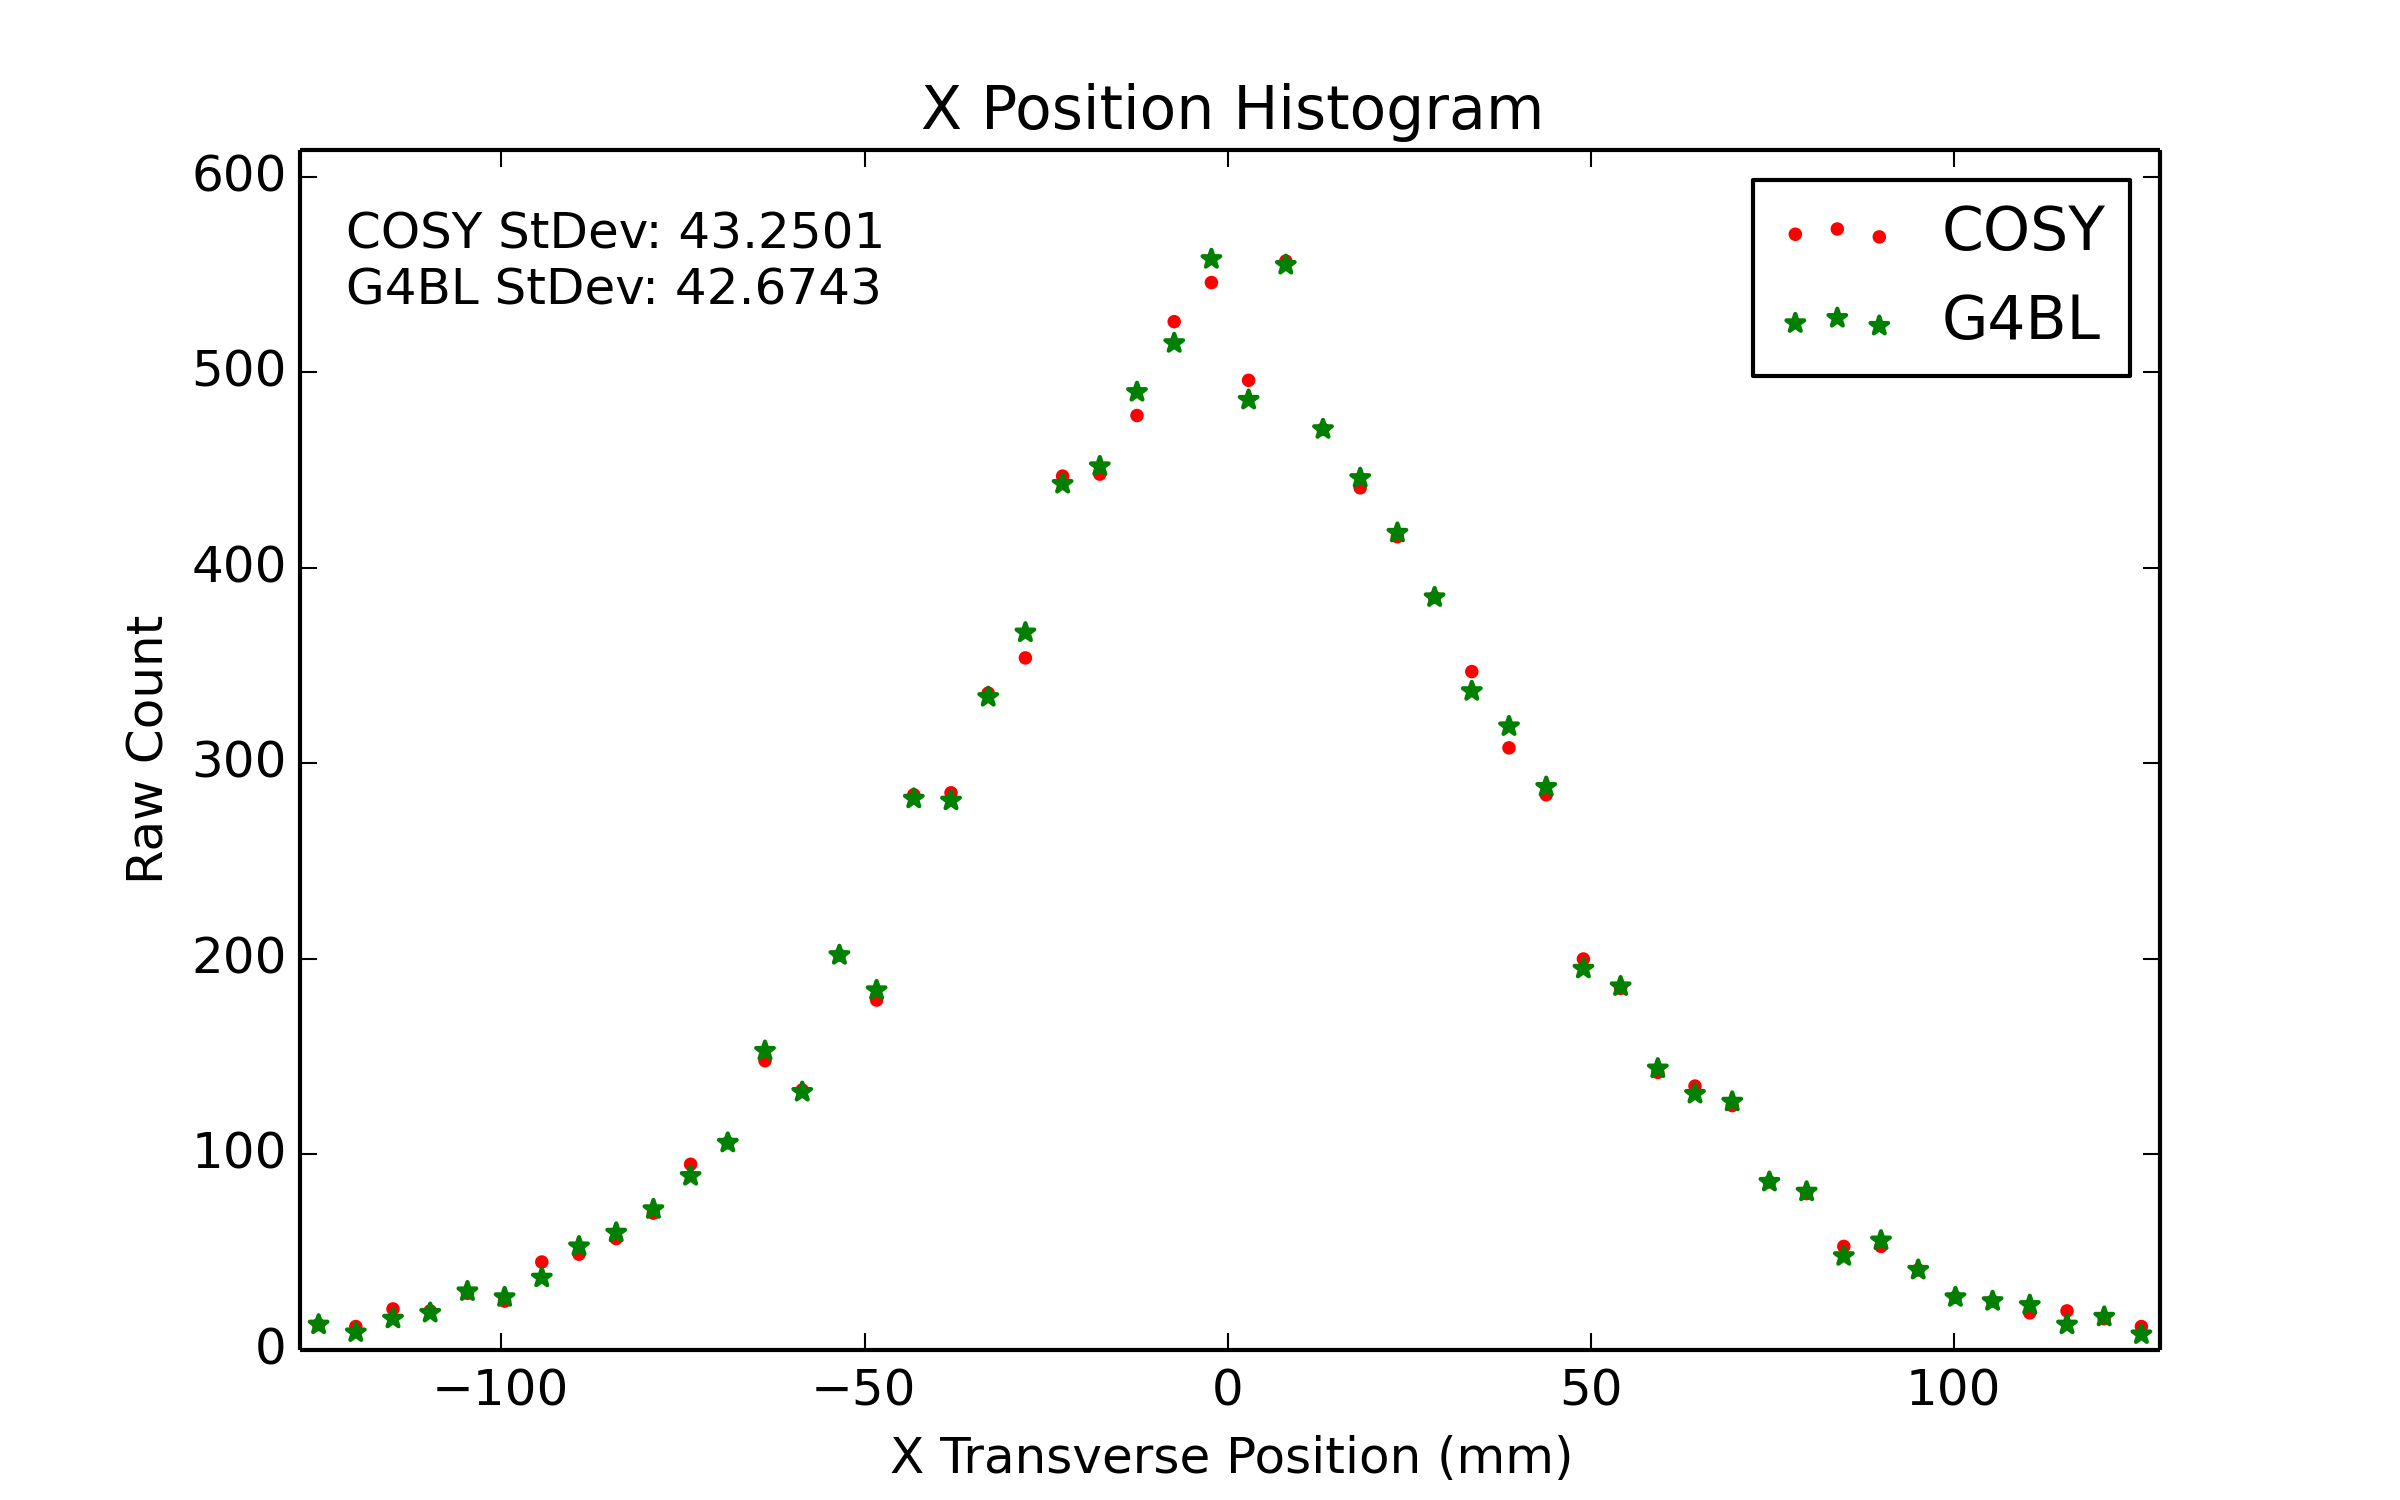
\includegraphics[width=85mm]{Figures/coil tests/xposition.png}
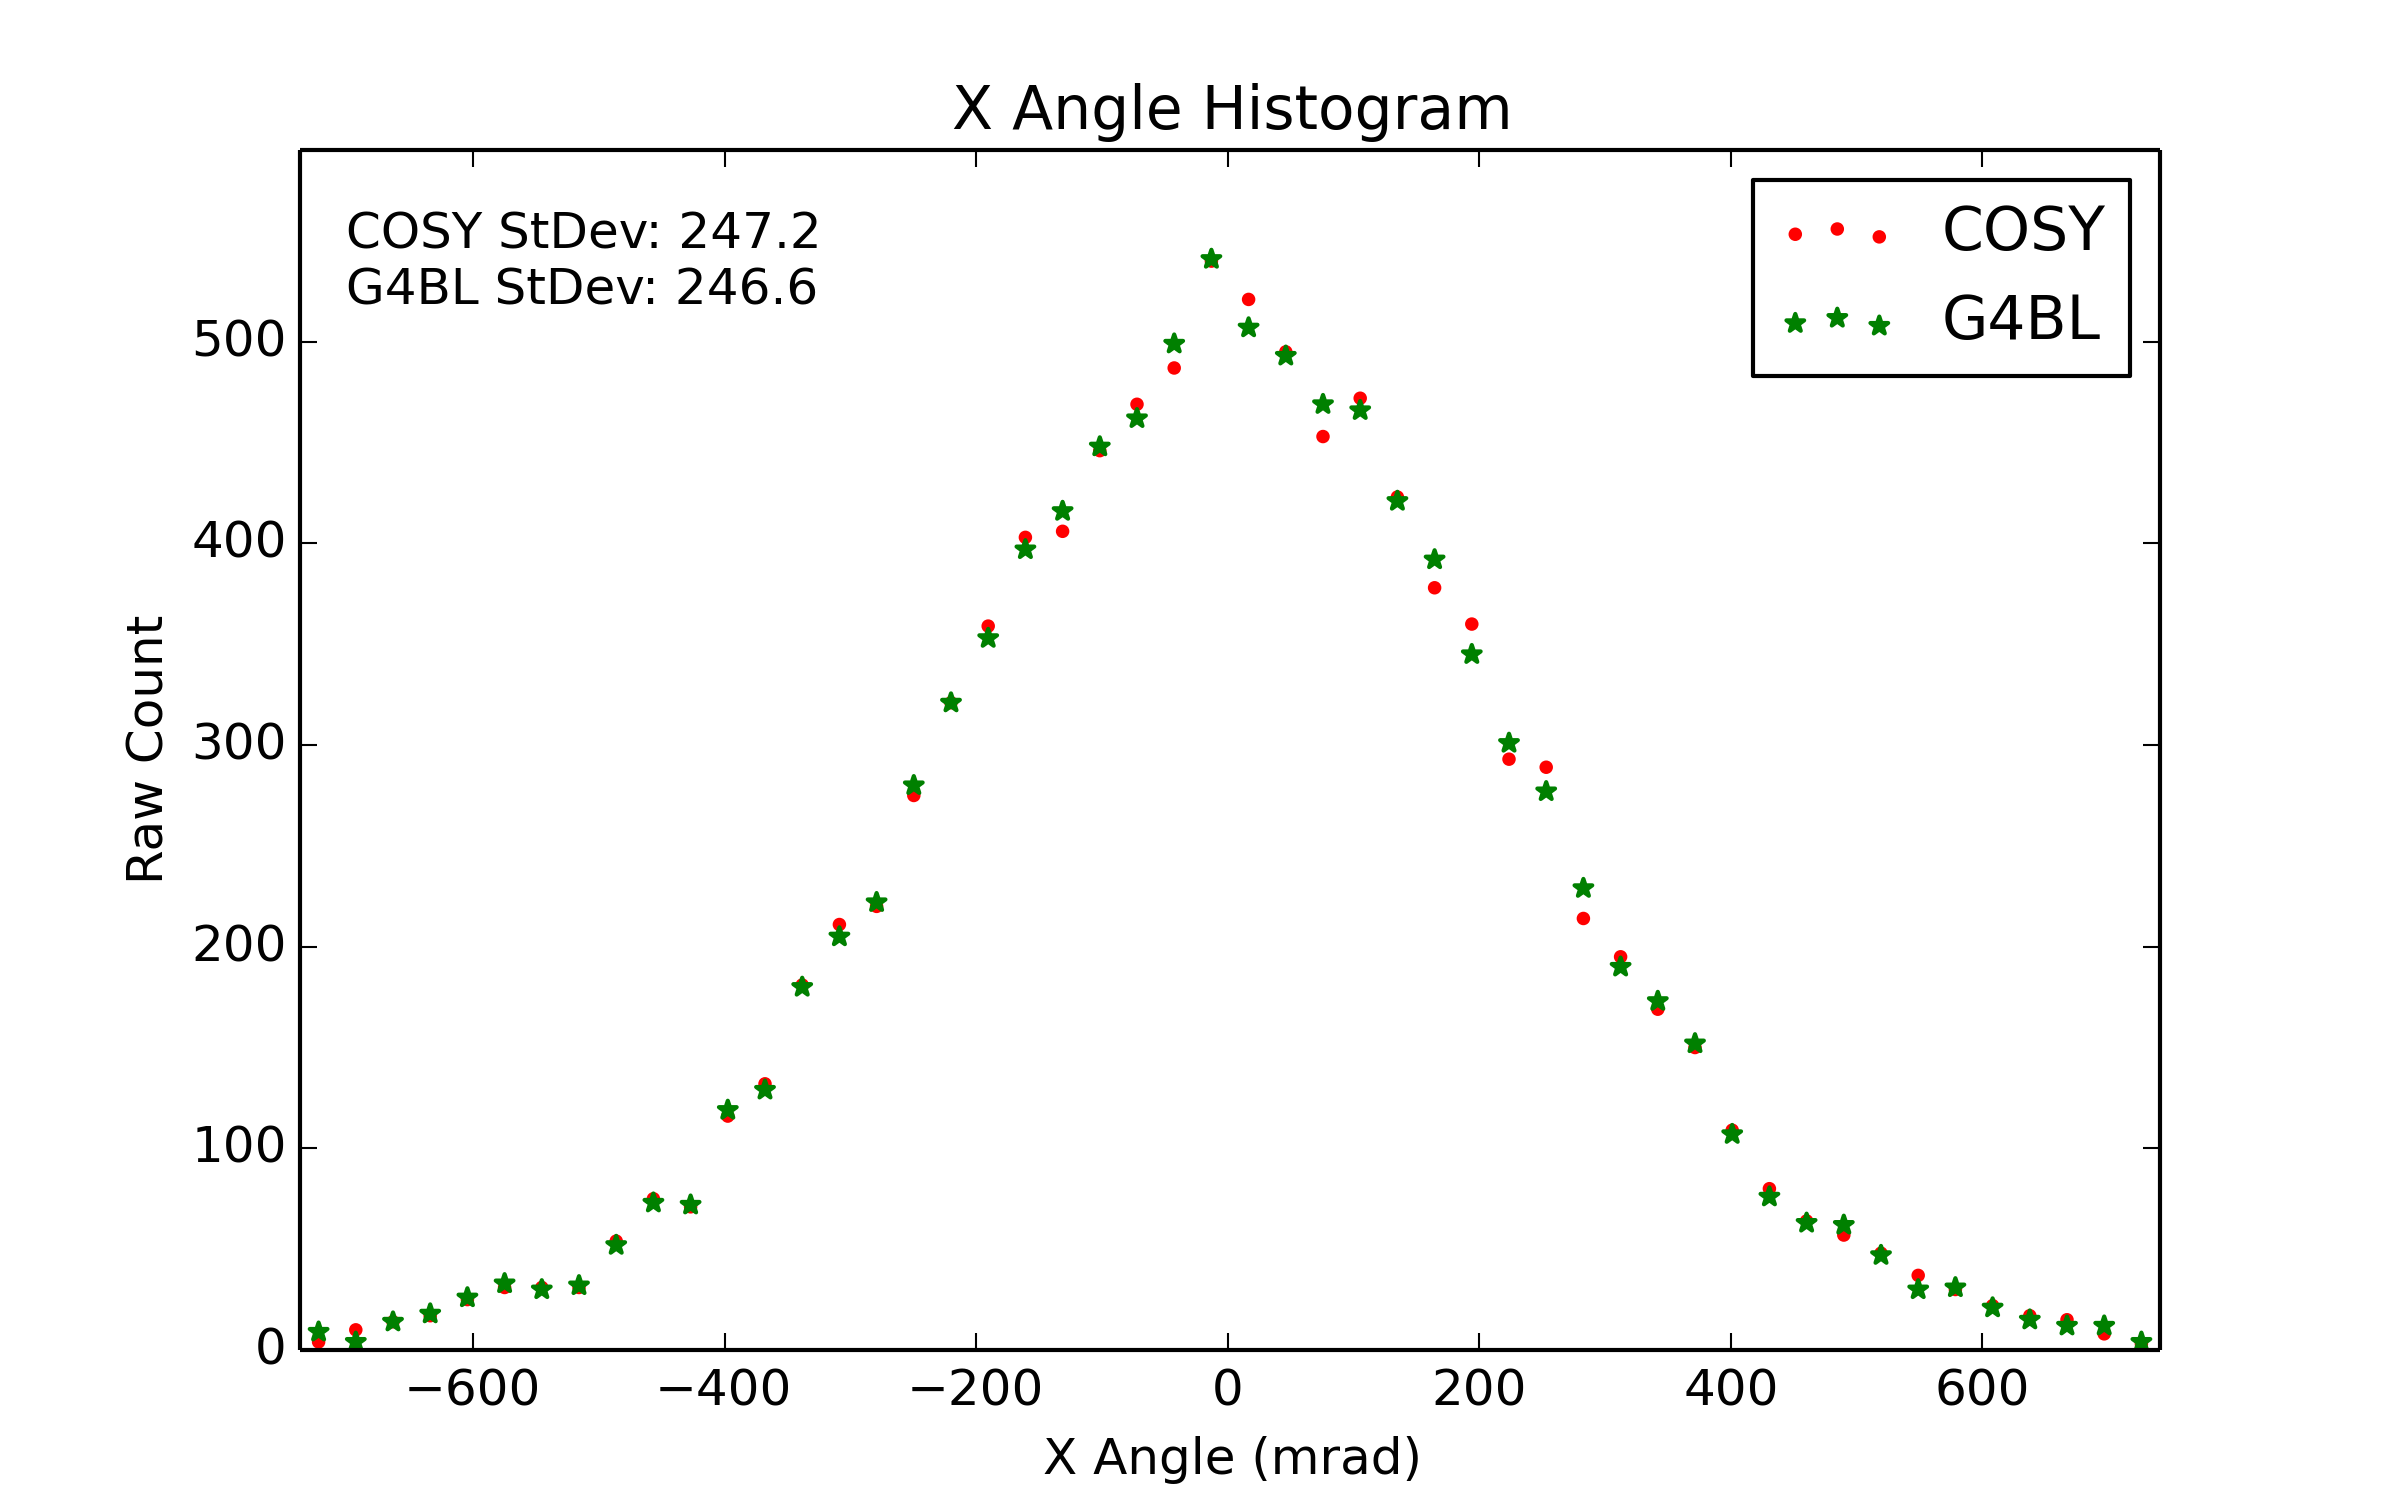
\includegraphics[width=85mm]{Figures/coil tests/xangle.png}
\caption{Position and angle histograms of initial distribution through MICE coil cell.}
\label{fig:mice_coil_histograms}
\end{figure}

For the flat lithium hydride absorber, the simulation in G4Beamline was carried out using the \texttt{tubs} routine. In COSY, the new routine \texttt{ABSPOLY} (polynomial absorber) was called. Details on the stochastic processes implemented by \texttt{ABSPOLY} can be found in \cite{ipac2015}. These results can be seen in Figure \ref{fig:mice_coil_absorber}.

\begin{figure}[h!]
\centering
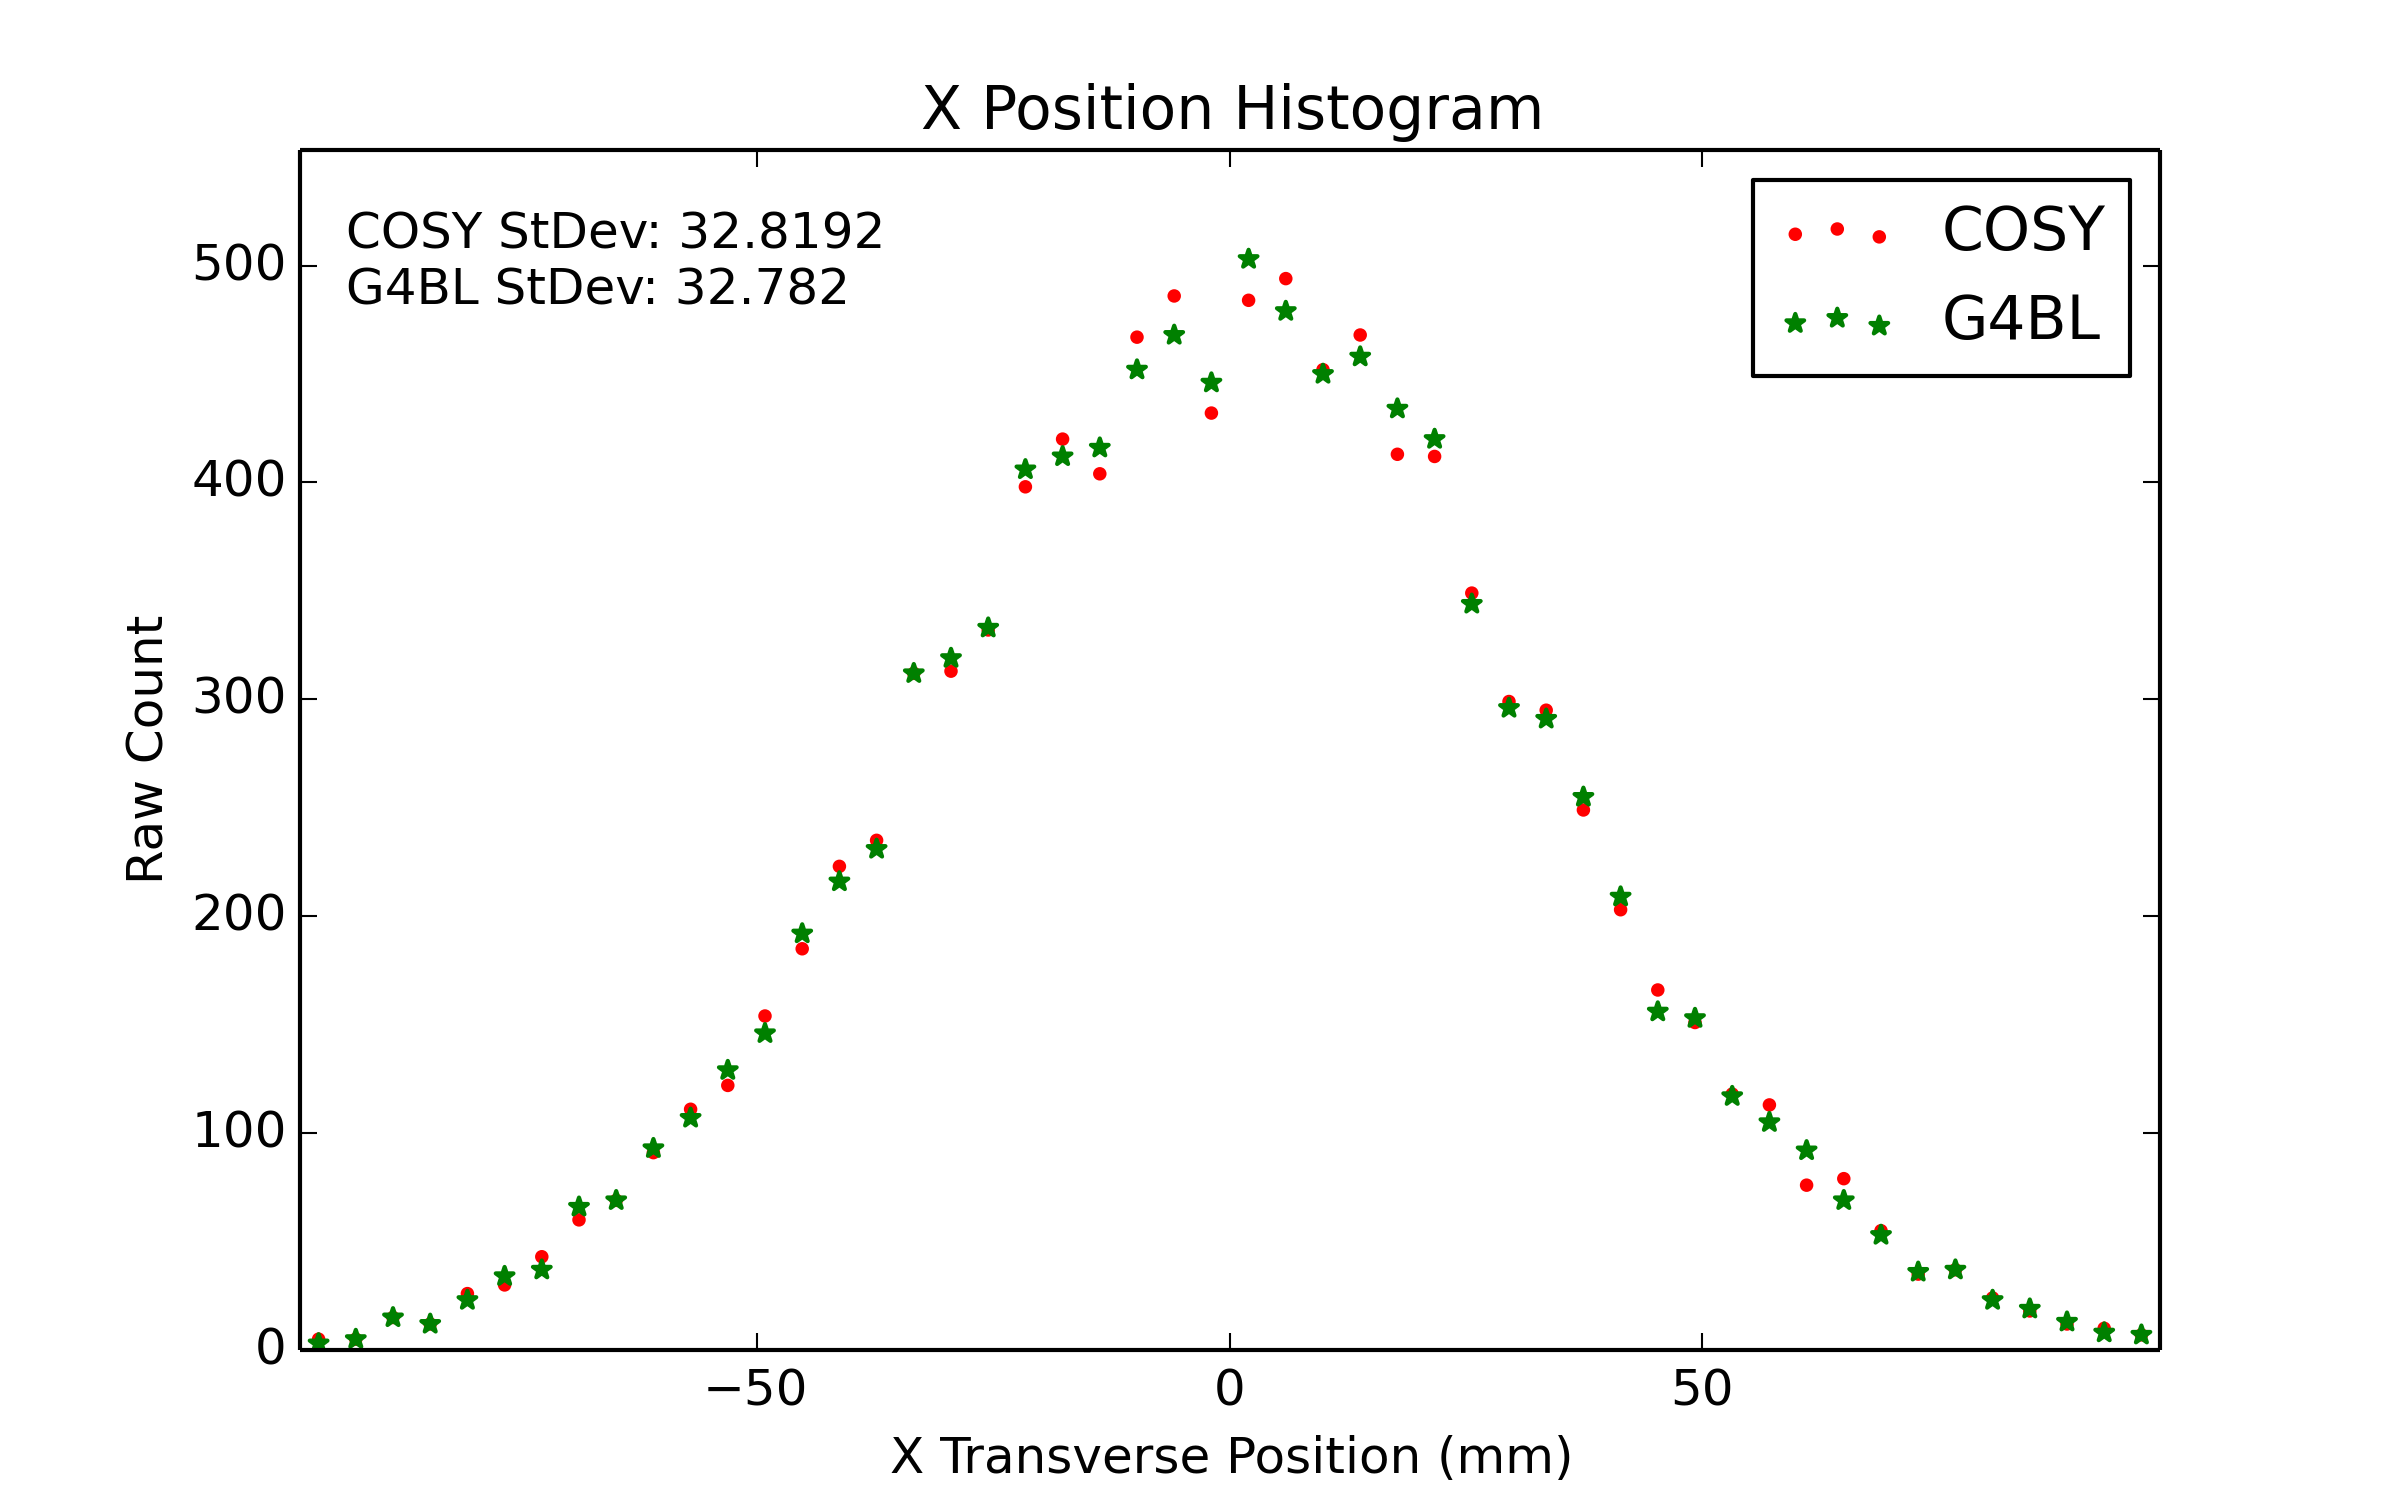
\includegraphics[width=85mm]{Figures/wedge tests (LiH)/xposition.png}
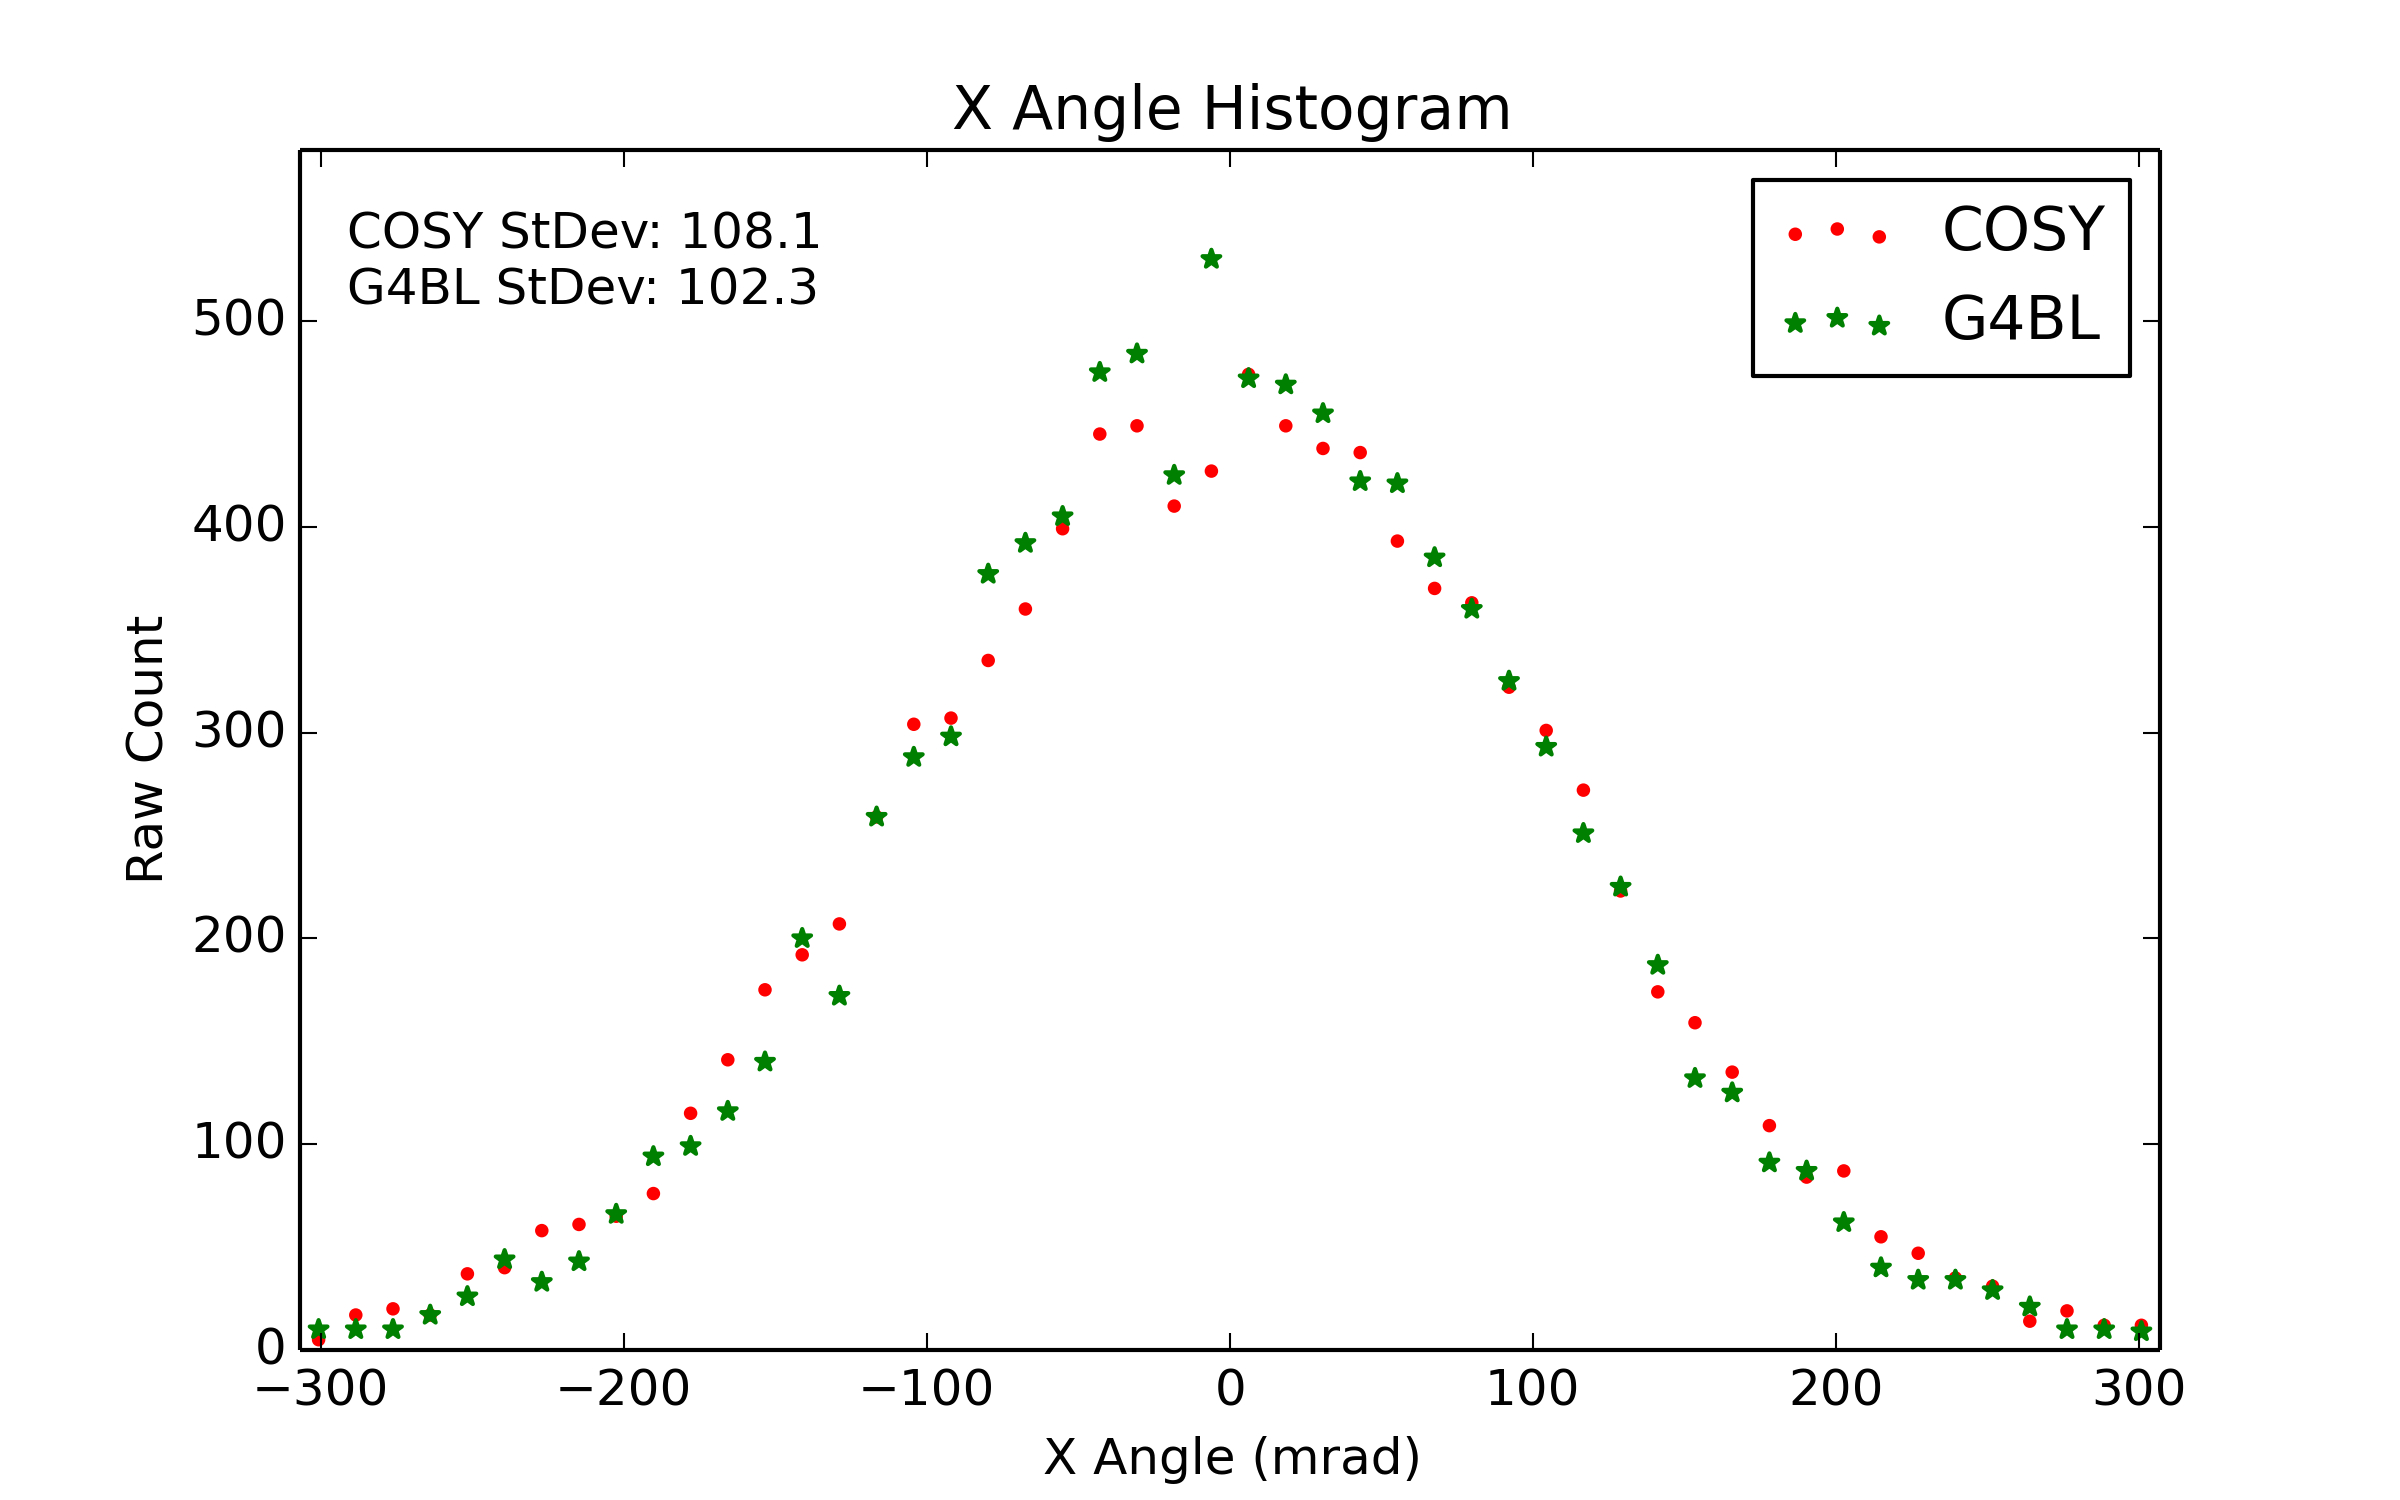
\includegraphics[width=85mm]{Figures/wedge tests (LiH)/xangle.png}
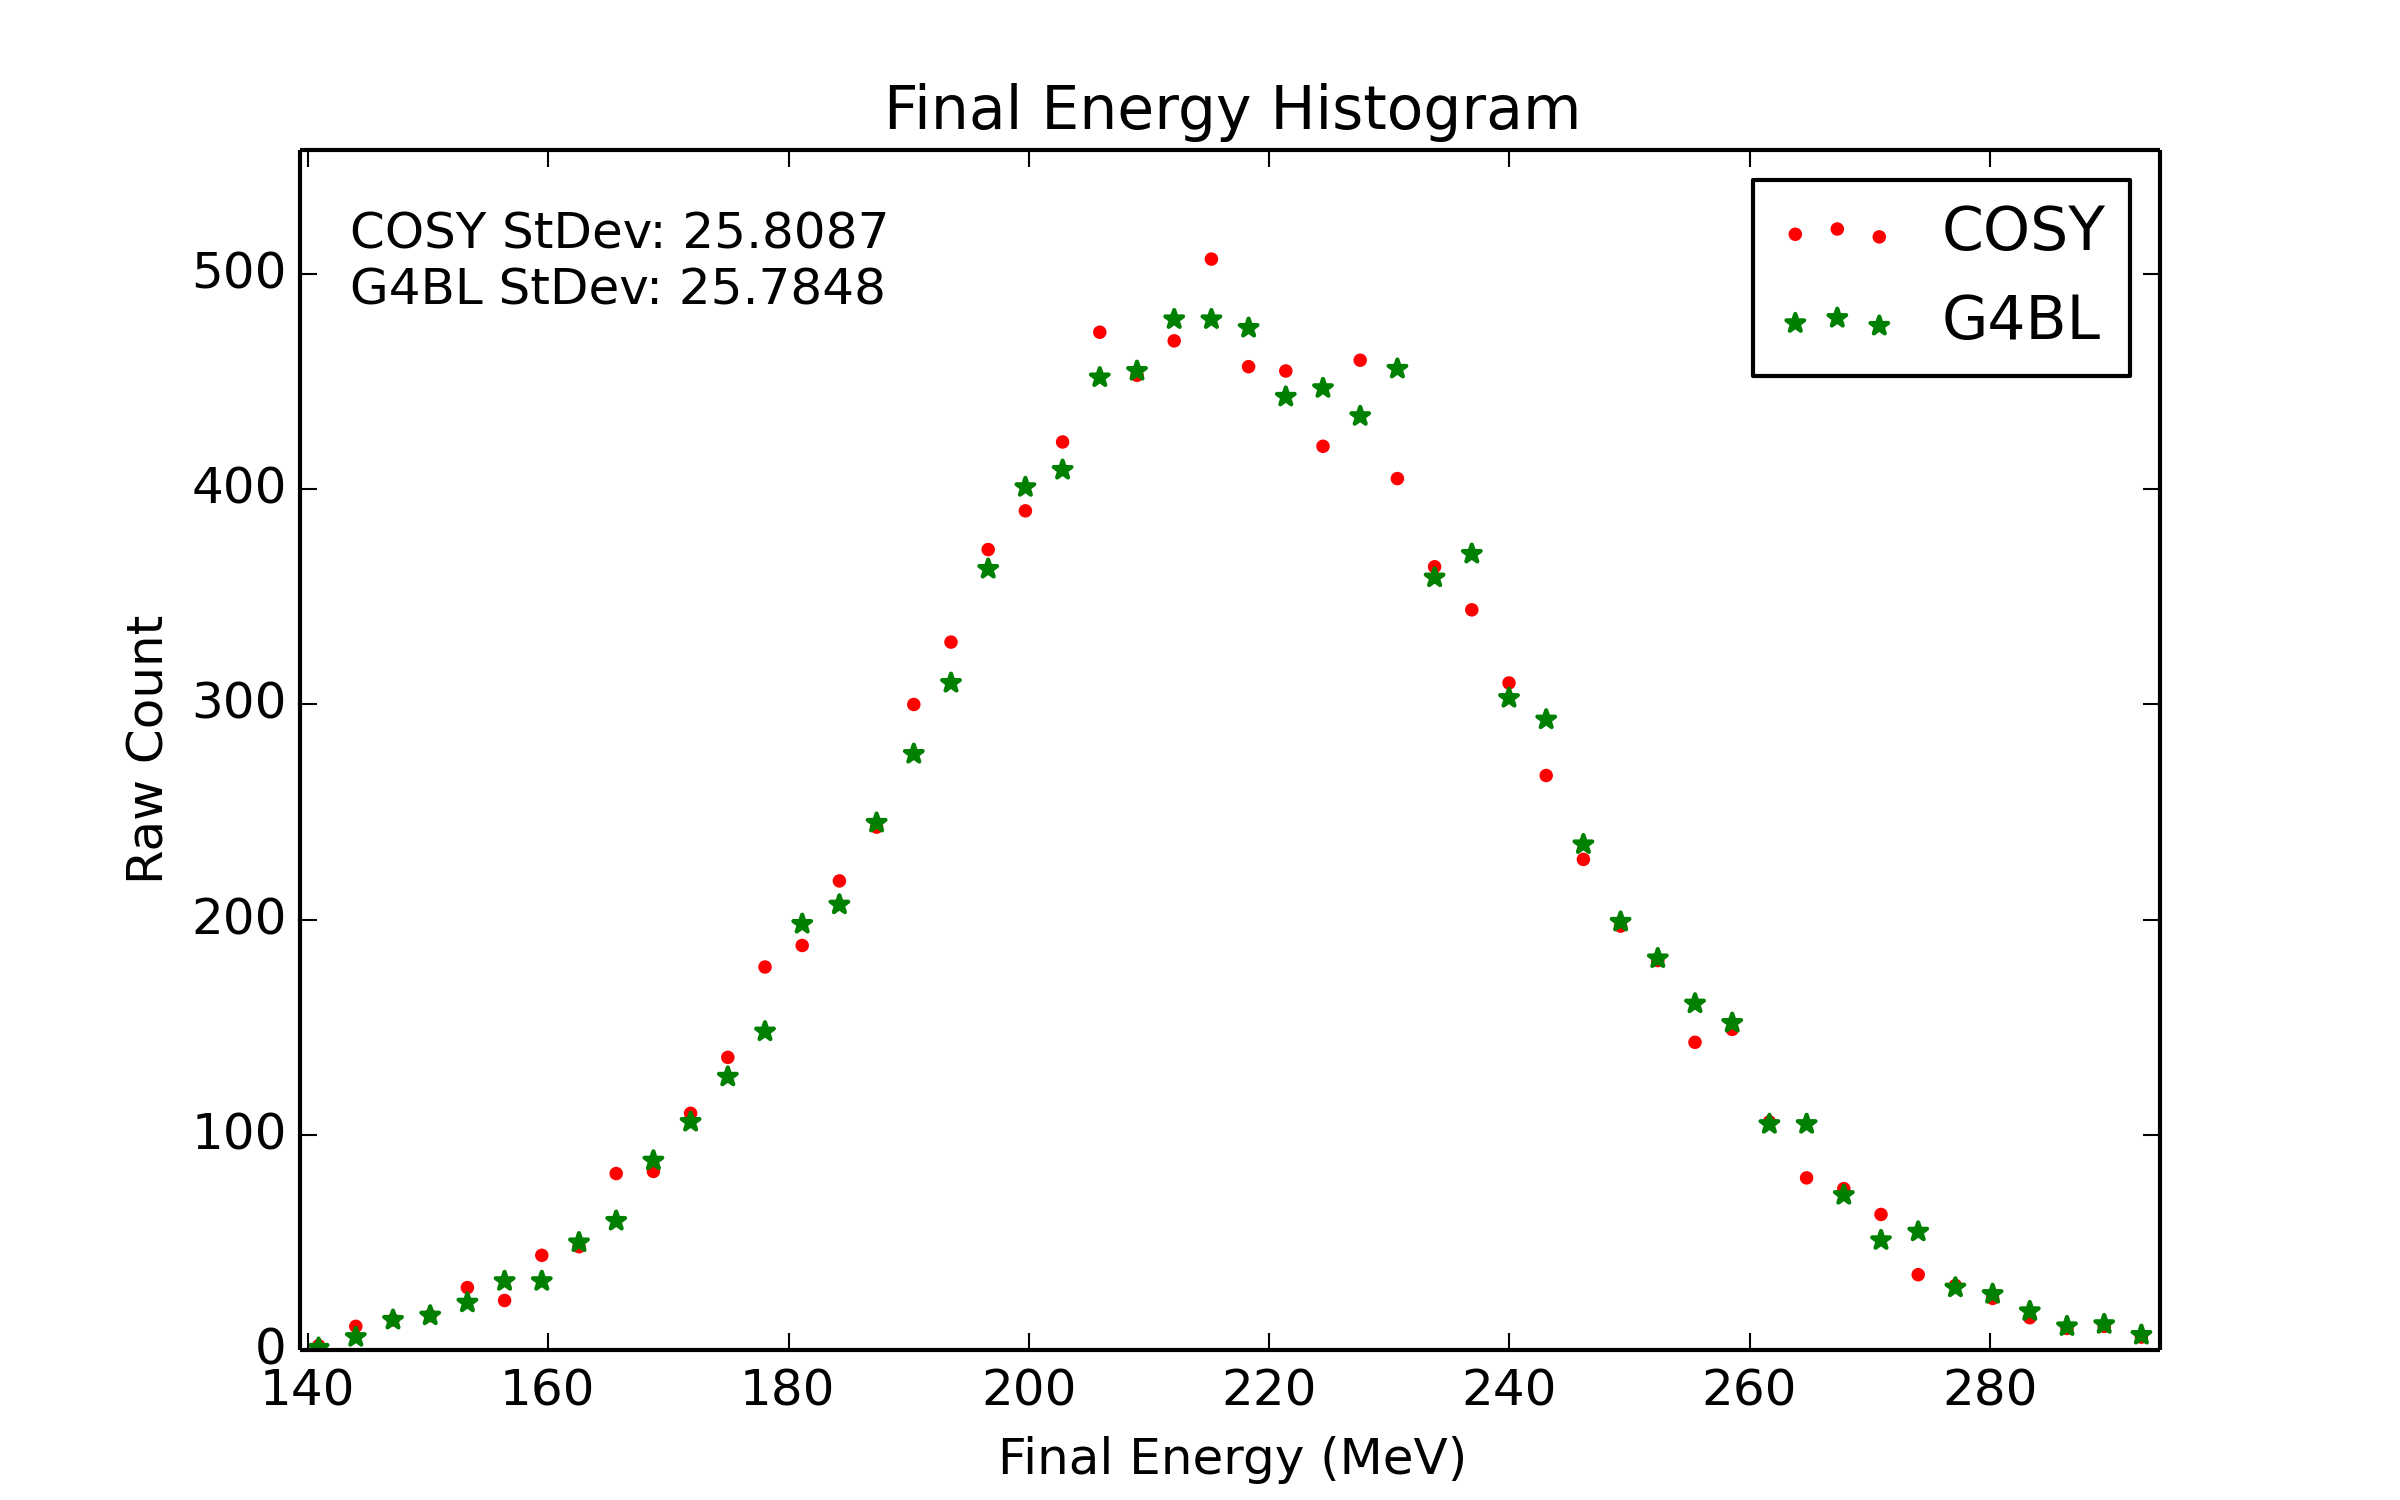
\includegraphics[width=85mm]{Figures/wedge tests (LiH)/energy.png}
\caption{Position, angle, and final energy histograms of initial distribution through MICE LiH absorber.}
\label{fig:mice_coil_absorber}
\end{figure}

\section{Current Challenges}
While the agreement in both the coils and the flat LiH absorber seem fair, the details on how to superimpose the two in COSY is still a subject for discussion. Additionally, some configurations use tilted coils. These coils generate a dispersion, and so a 90$^{\circ}$ wedge absorber is used. However, COSY does not currently have a way to arbitrarily tilt an arbitrary arrangement of coils, and so such a routine is being researched. Finally, the differences in the COSY RF kick versus the G4Beamline pillbox model need to be explored and addressed. This could also be solved by implementing a new lattice element in COSY.

\bibliography{bib}{}
\bibliographystyle{plain}
\end{document}